\documentclass[mathserif]{beamer}

\mode<presentation> {

\usetheme{Madrid}

}
\usepackage{stmaryrd}
\usepackage{listings}
\usepackage{graphicx} % Allows including images
\usepackage{booktabs} % Allows the use of \toprule, \midrule and \bottomrule in tables

\newcommand{\bis}[1]{\begin{itemize}\setlength{\itemsep}{#1}}

\begin{document}

\title[Cyberinfrastructure]{Detecting Ocean Eddies is Sea Surface Height Data}

\author[Matt Le]{Matt Le}

\institute[RIT]{Rochester Institute of Technology}
\date{\today} % Date, can be changed to a custom date

%Title
\begin{frame}
\titlepage
\end{frame}

%Eddies
\begin{frame}{Ocean Eddies}
\begin{tabular}[c]{p{.5\textwidth}p{.45\textwidth}}
 \begin{itemize}
 \item Spinning pools of water
\item Transport heat, salt, and nutrients

 \end{itemize}
 &
 \vspace{2pt}%
 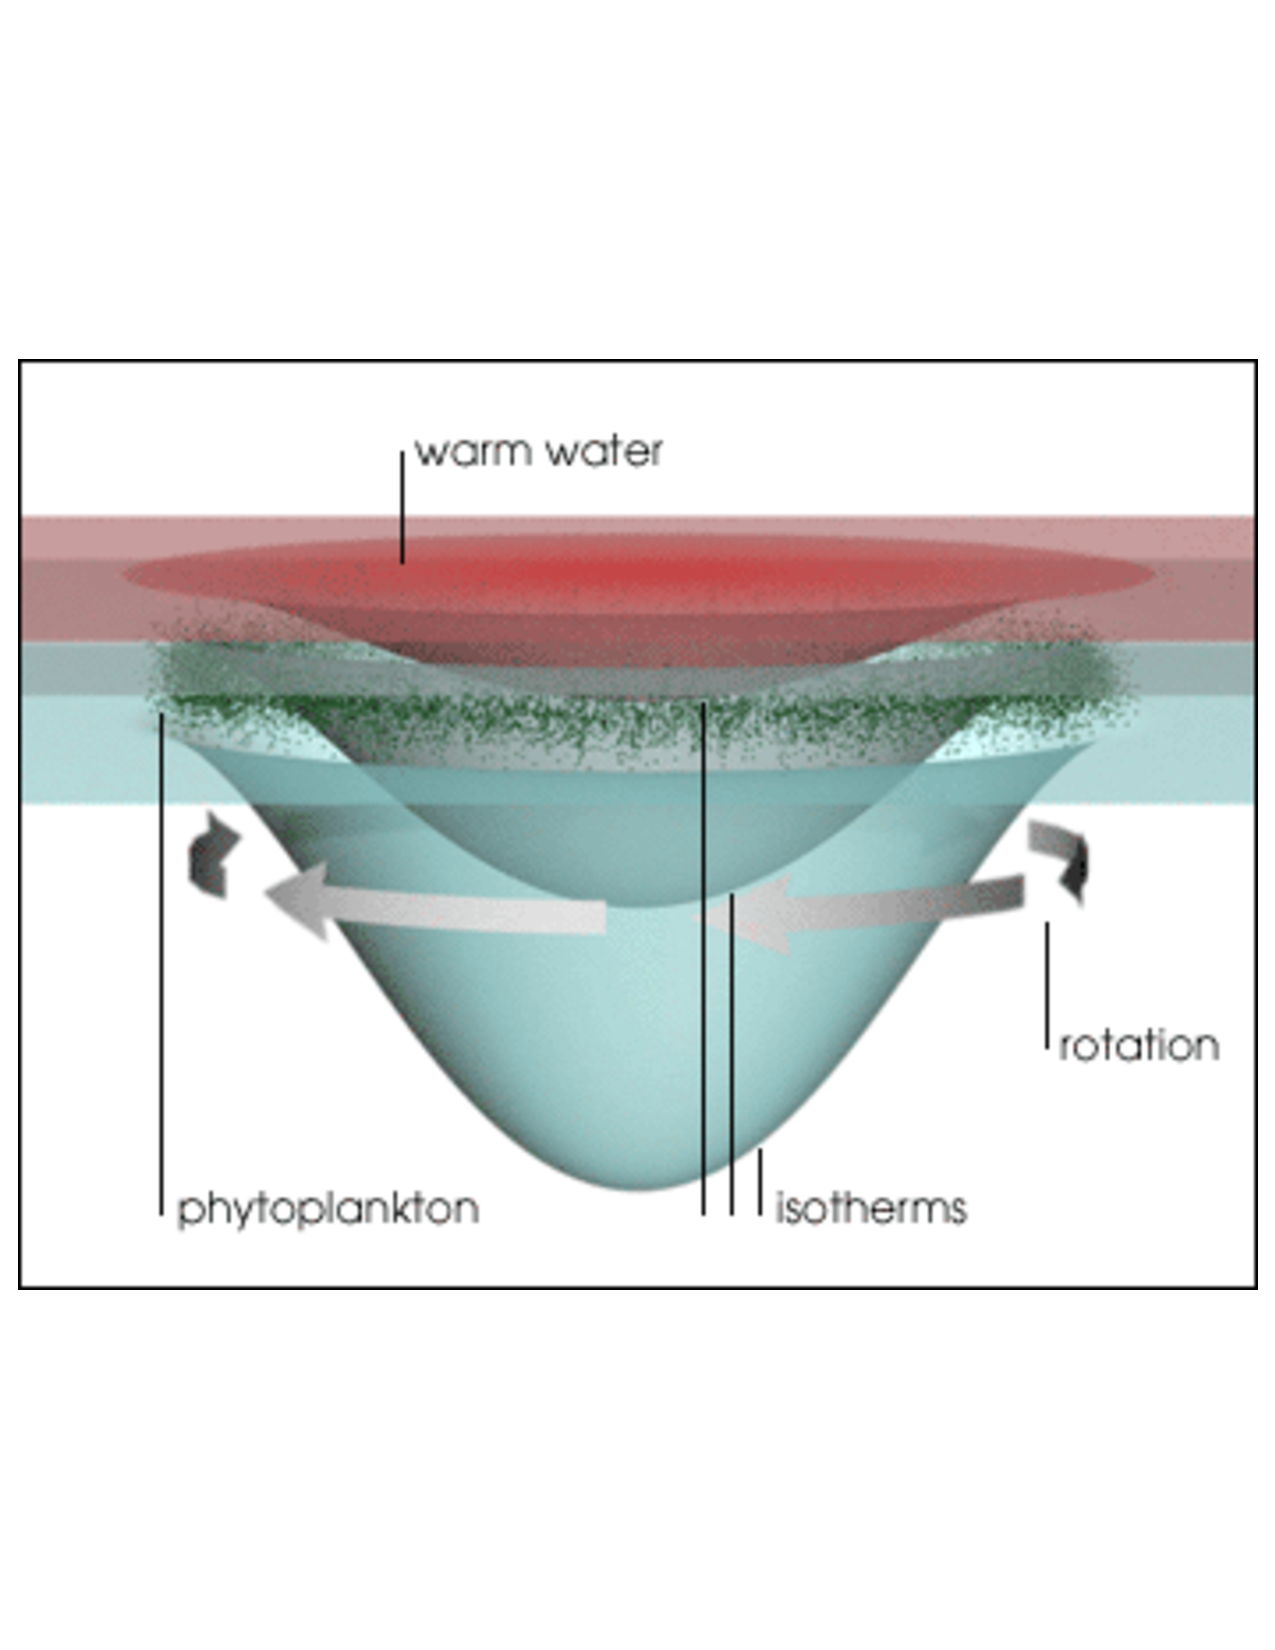
\includegraphics[scale=.2]{figures/eddy_render.pdf}
 \end{tabular}
\end{frame}

%Global Eddies
\begin{frame}
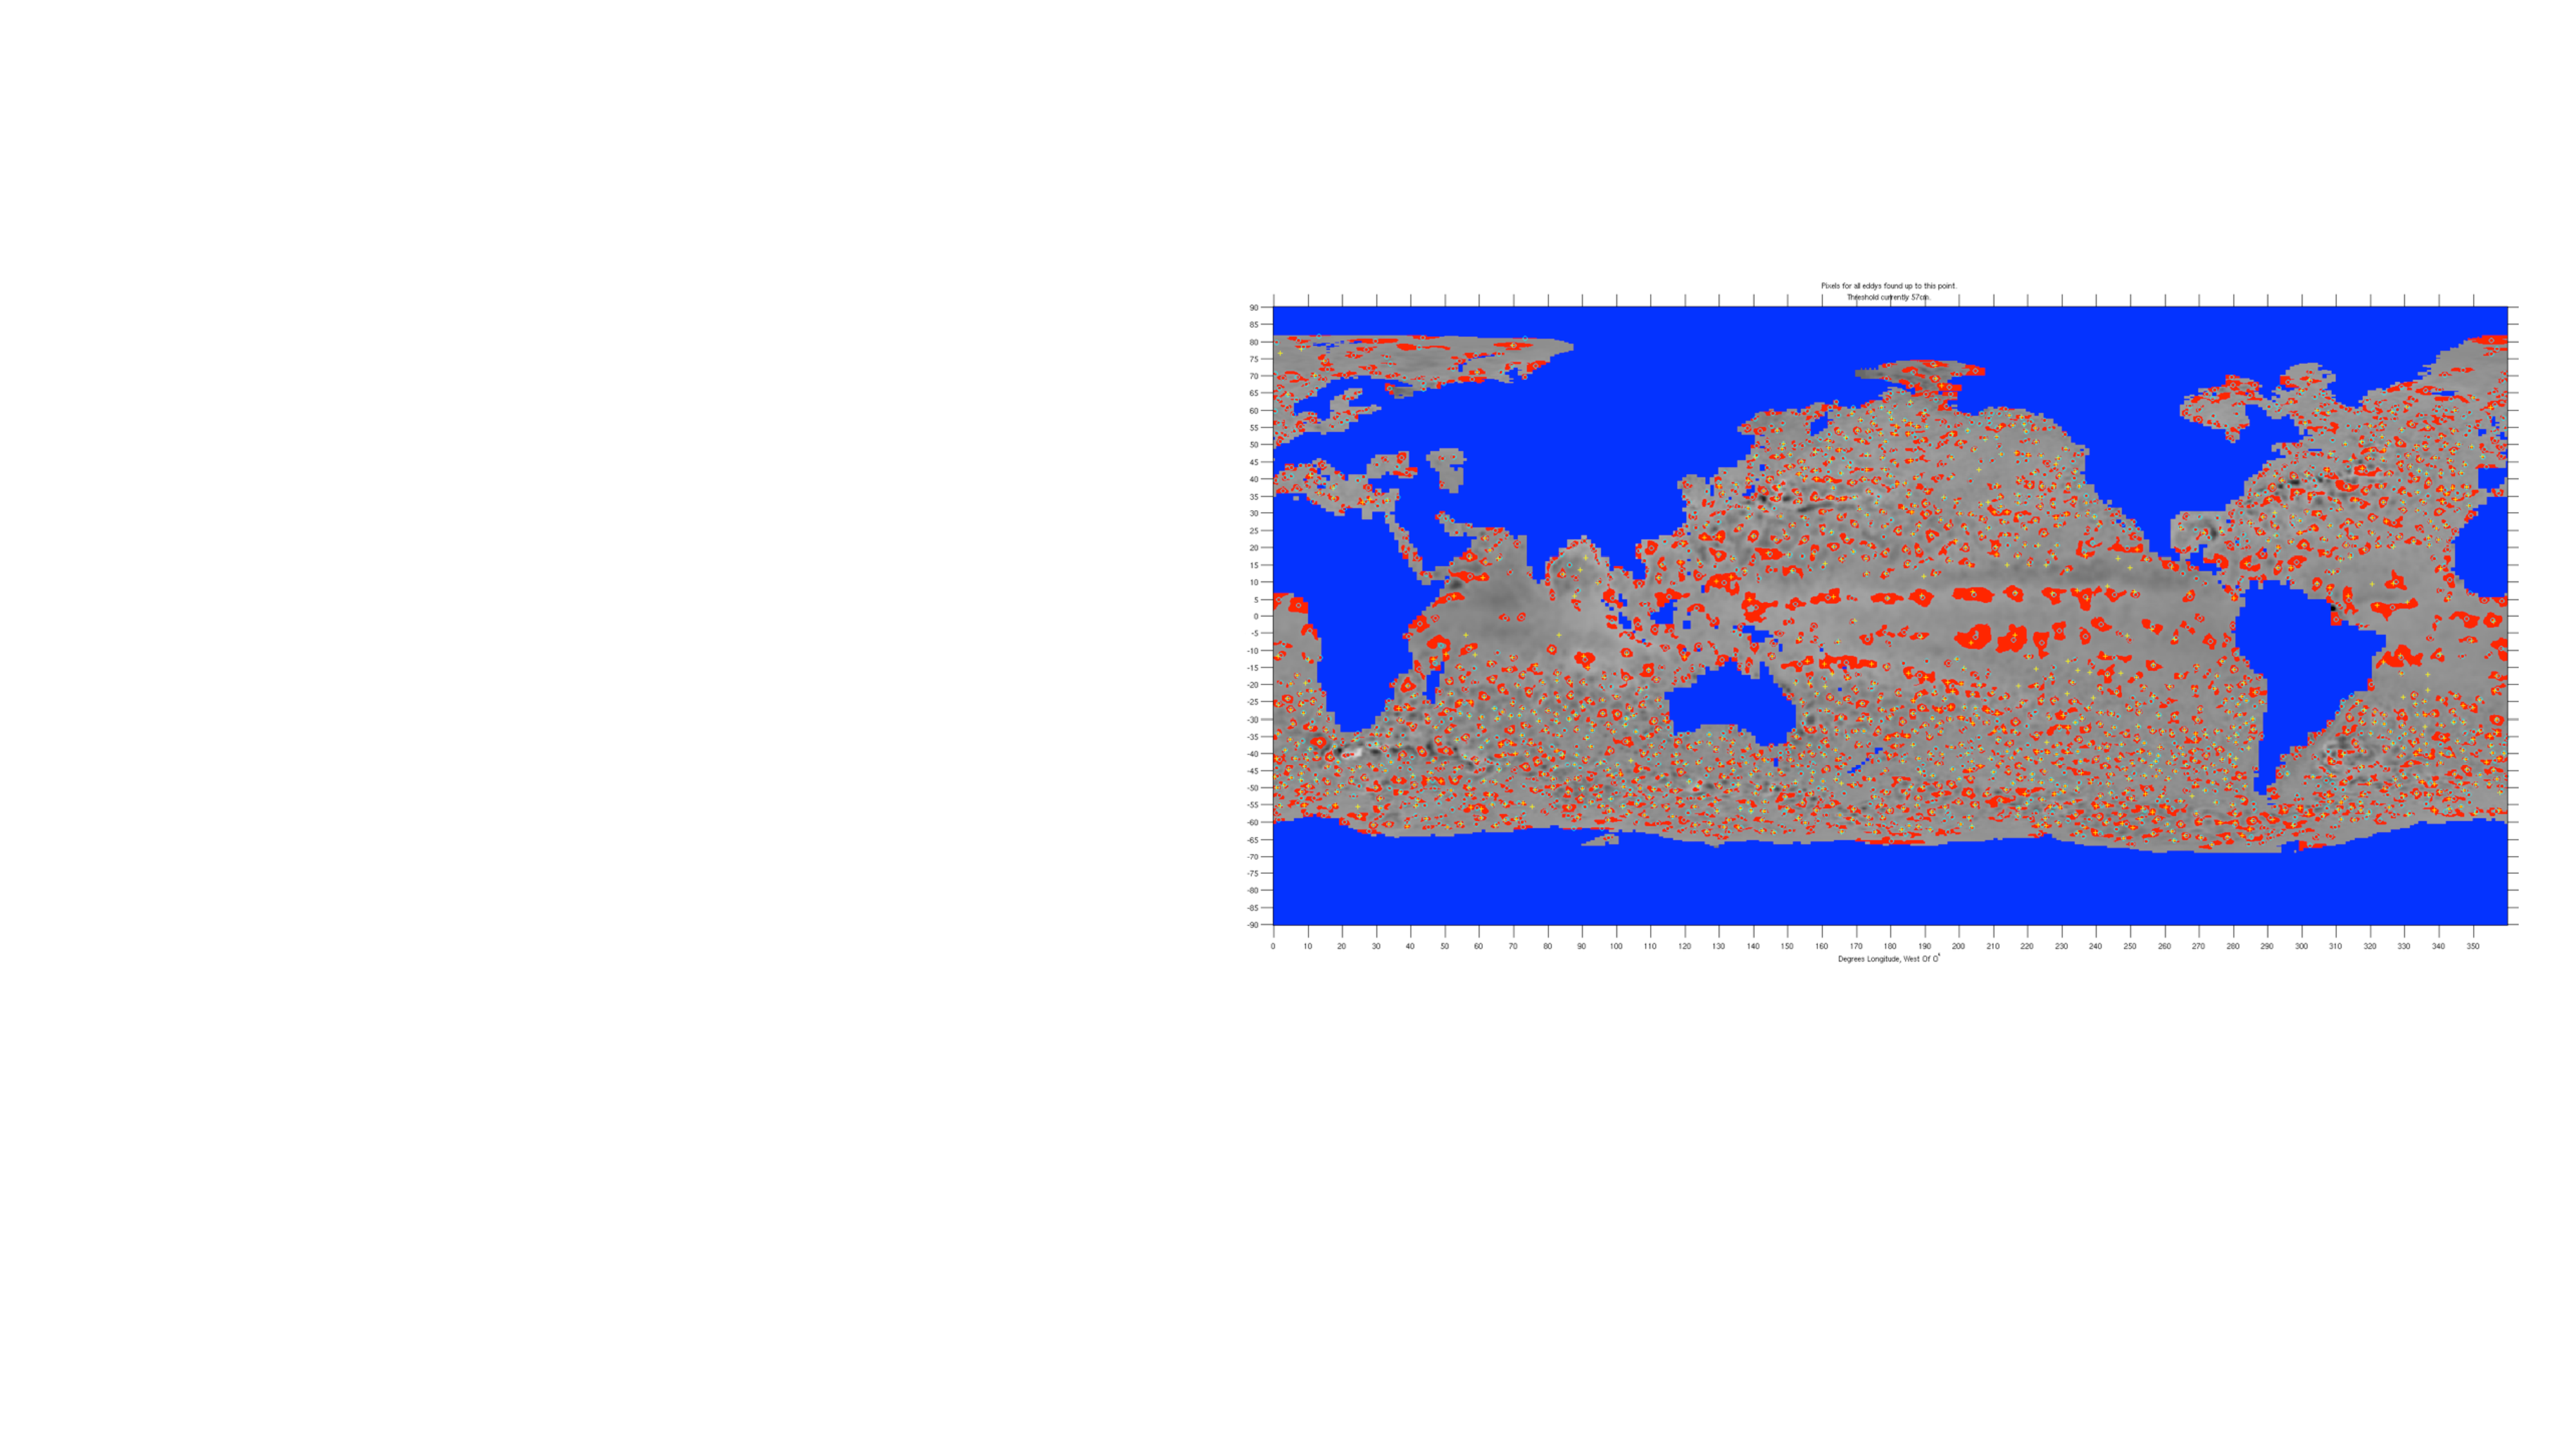
\includegraphics[scale=.32]{figures/globalEddies.pdf}
\end{frame}

%Data
\begin{frame}{The Data}
\begin{itemize}
\item 721 X 1440 X 954
\end{itemize}
\begin{figure}
\centering
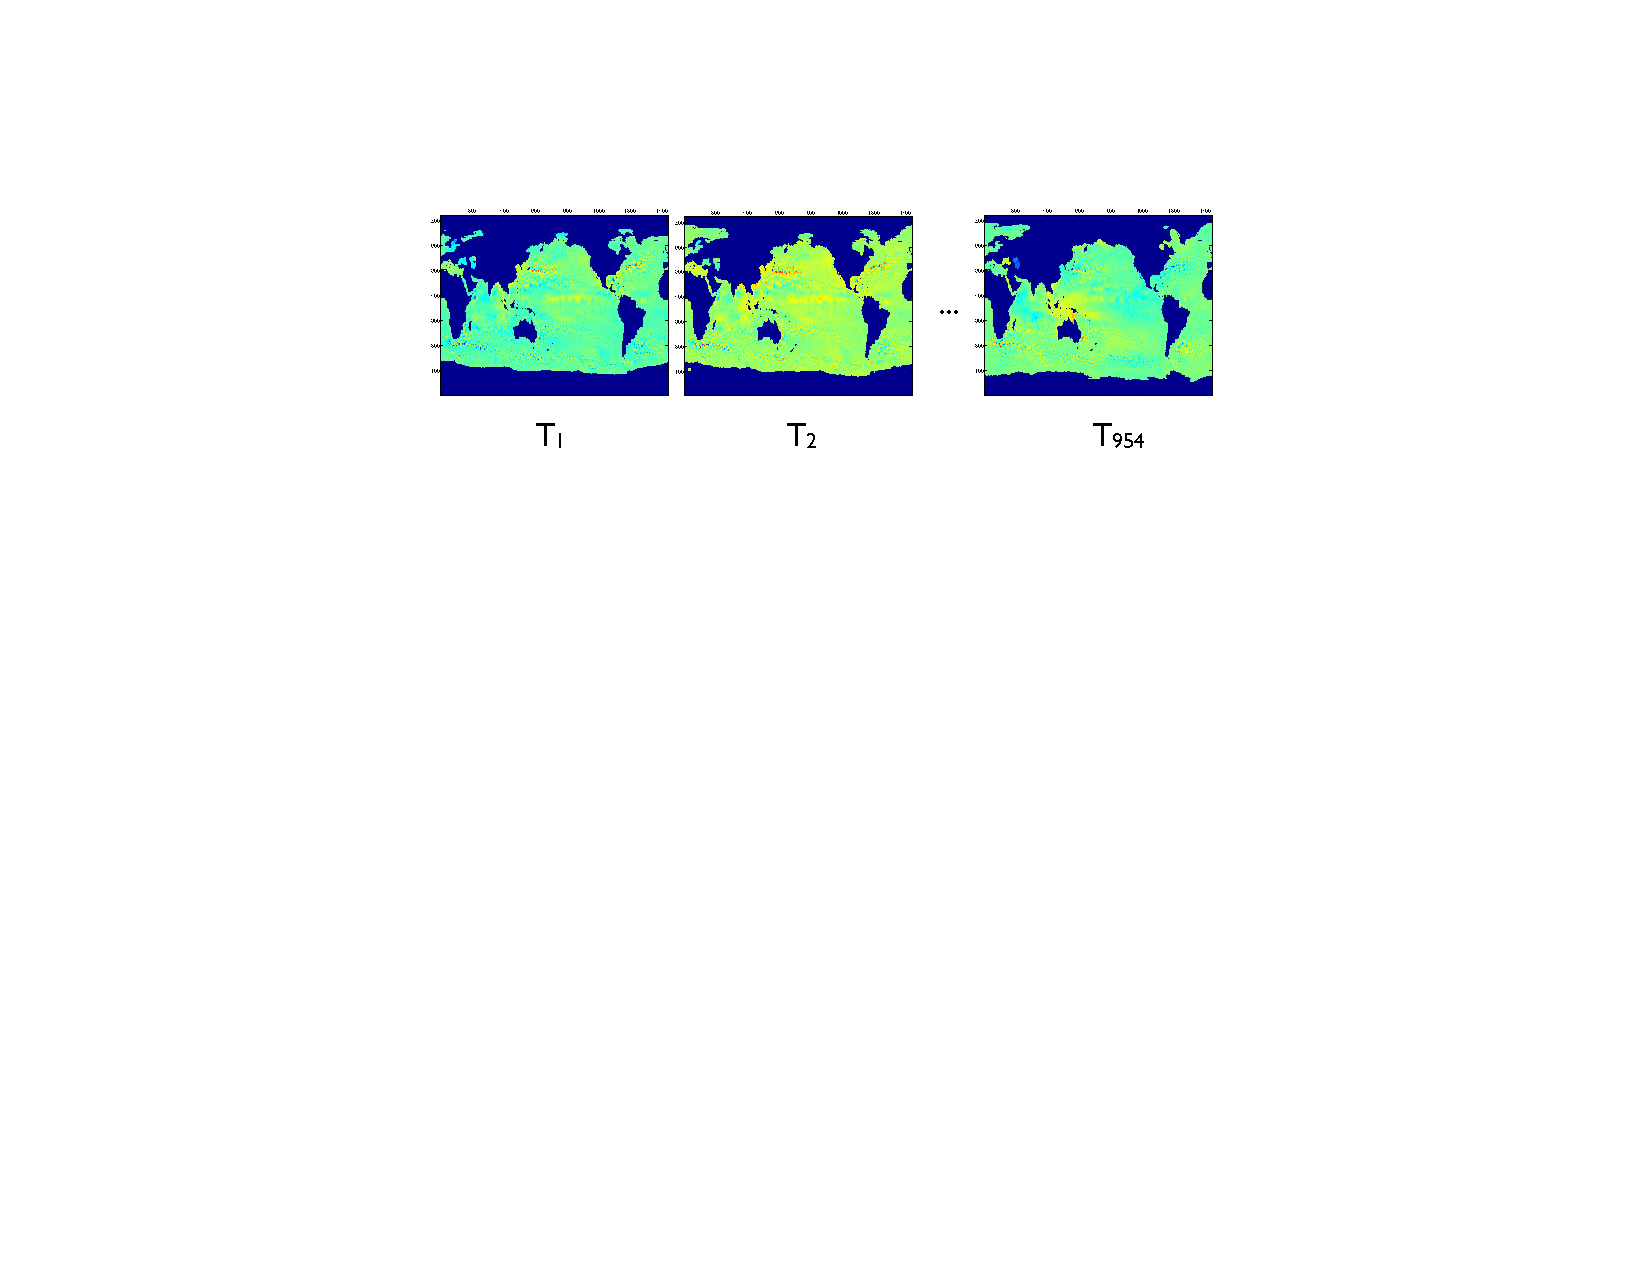
\includegraphics[scale=.8]{figures/sshMaps.pdf}
\end{figure}
\end{frame}

%Algorithm
\begin{frame}{Detecting Eddies}
\begin{tabular}[c]{p{.5\textwidth}p{.45\textwidth}}
 \begin{itemize}
 \item Iteratively threshold data
 \item Search for connected components
 \end{itemize}
 &
 \vspace{2pt}%
 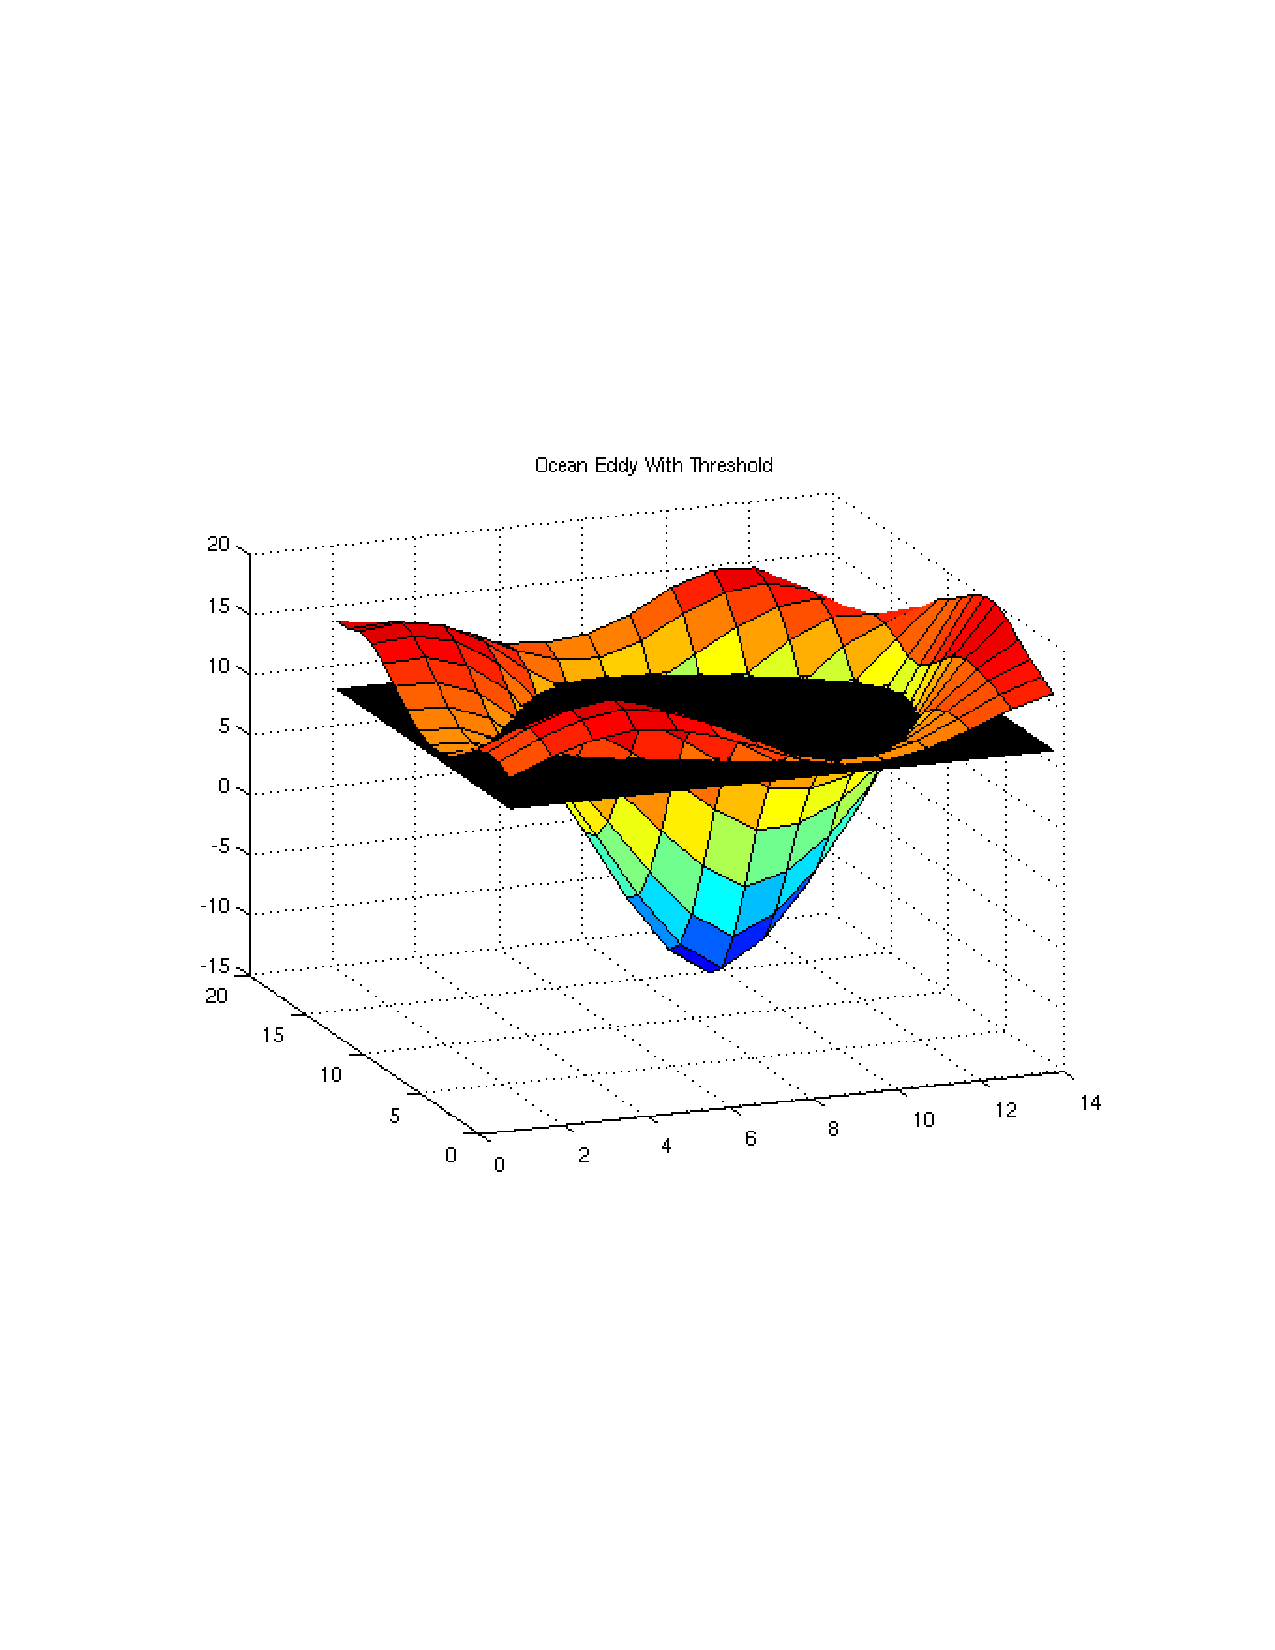
\includegraphics[scale=.35]{figures/eddyWithThreshold.pdf}
 \end{tabular}
\end{frame}

%Parallel implementation
\begin{frame}{Implementation}
\begin{itemize}
\item Spawn a thread for each physical processor
\item Each thread gets the next week to be processed from a global variable
\begin{itemize}
\item Read the given week's SSH data form a file
\item Process it
\item Write the results to a file and repeat
\end{itemize}

\end{itemize}
\end{frame}

\begin{frame}{Scalability}
\begin{figure}
\centering
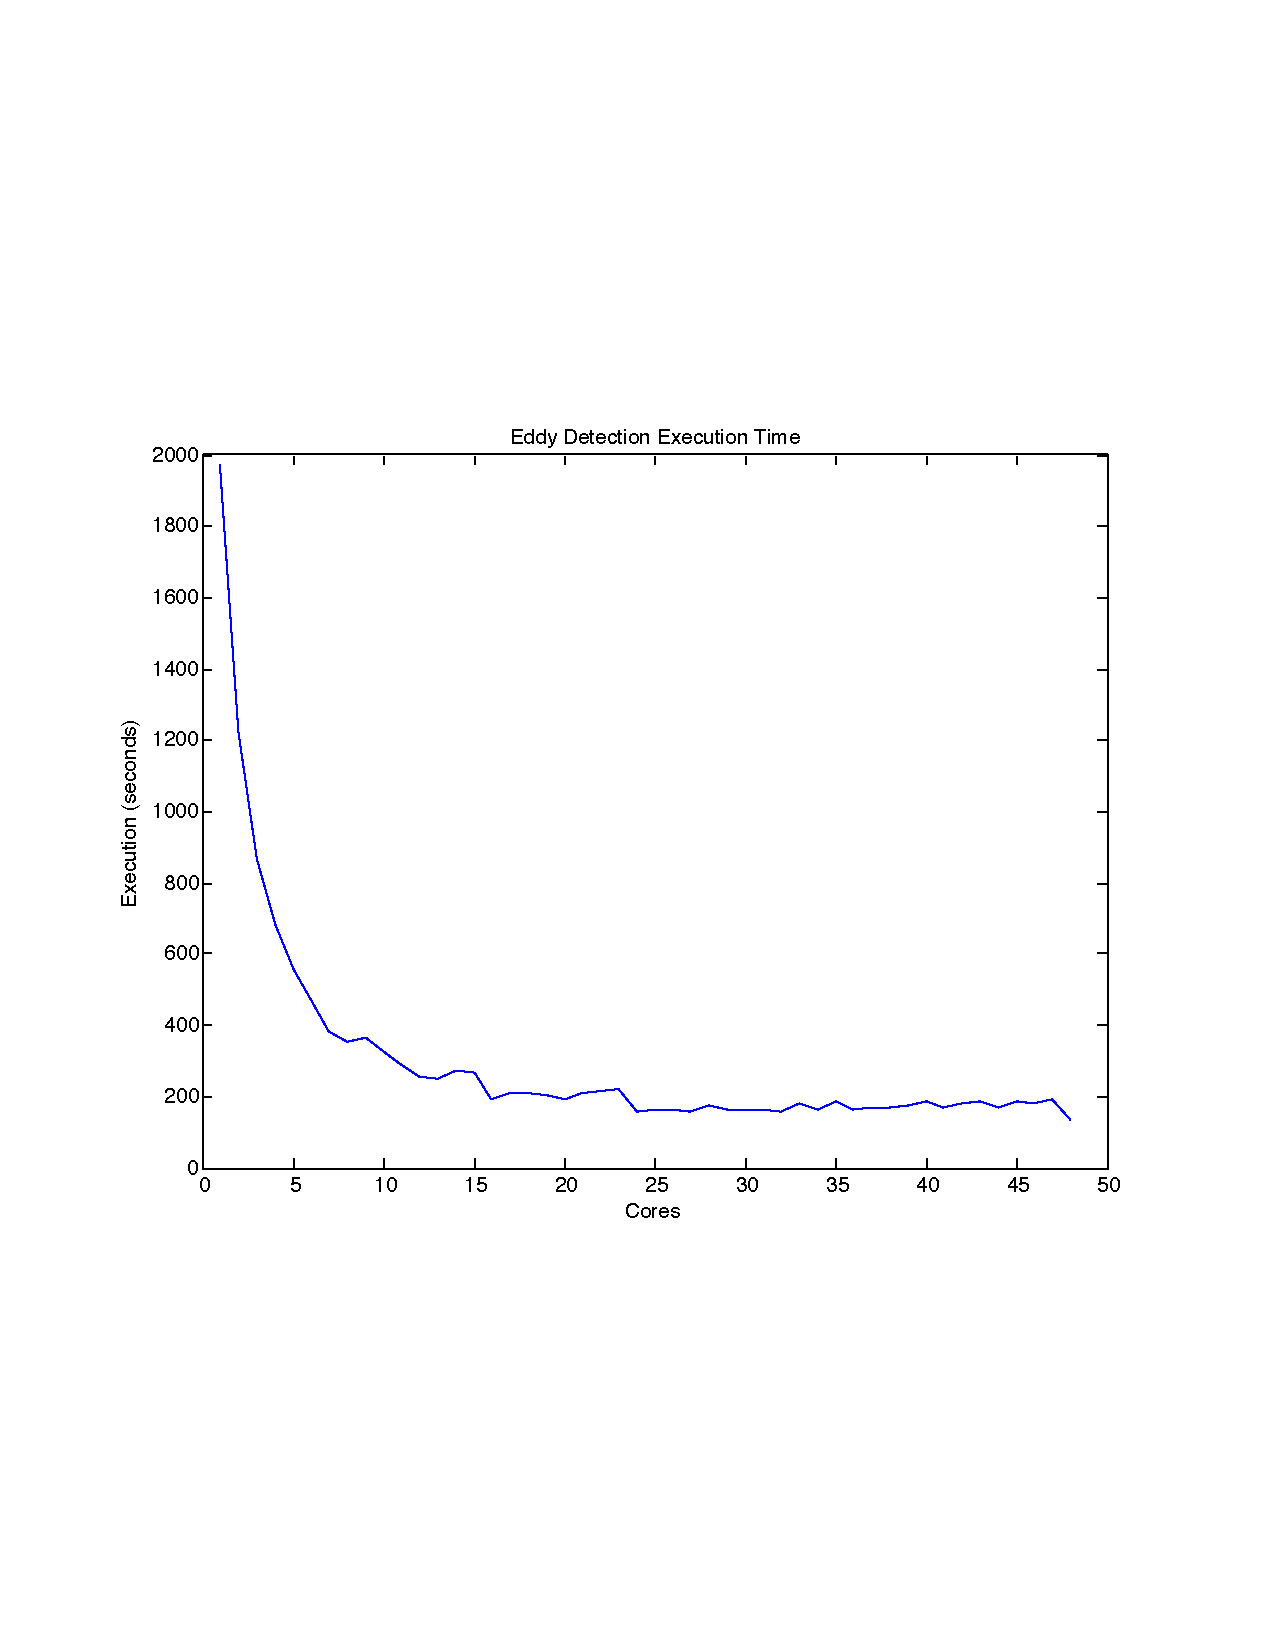
\includegraphics[scale=.5]{figures/times.pdf}
\end{figure}
\end{frame}

\begin{frame}[fragile]{Performance: Java vs. MATLAB}
\begin{itemize}
\item Java is much faster
\item 5.1733 hours vs. 32.8833 minutes
\end{itemize}

\end{frame}


\begin{frame}{Questions}
\centering
\large{Questions?}

\end{frame}

\end{document}




